%%
% La siguiente plantilla esta basada en el siguiente enlace:
% http://academic.reed.edu/physics/courses/Physics332.s08/reports.html
% La plantilla original puede descargarse de ese sitio
% Se dejo parte del texto original en inglés para ilustar el uso de la plantilla
% Se hicieron algunas modificaciones para ajustar el idioma y otros detalles para 
% completar un reporte técnico breve pero muy puntual
% Modificación Inicial: Marco Aurelio Nuno Maganda - 11/SEP/2014
% 
% Enlace a la documentación del tipo de documento base (revtex4)
% http://mirror.hmc.edu/ctan/macros/latex/contrib/revtex/doc/latex/revtex/source/revtex4-1.pdf
%
% En algunas distribuciones es necesario instalar el paquete texlive-publishers
%
%\documentclass[letterpaper,aps,twocolumn,pre,nofootinbib]{revtex4}
%\documentclass[twocolumn]{article}
\documentclass[conference]{IEEEtran}

\usepackage[spanish]{babel}
\usepackage{amsmath,amssymb,amsfonts,amsthm}
\usepackage{graphicx}
%\usepackage{bbm}
\usepackage[utf8]{inputenc} % Caracteres en Español (Acentos, ñs)
\usepackage{url} % ACENTOS
\usepackage{hyperref} % Referencias
\usepackage{subfig}
\usepackage{lipsum}
\usepackage{balance}
\usepackage{float}


%%%%%%%%%%%%%%%%%%%%%%%%%%%%%%%%%%%%%%%%%%%%%
% PARCHE PARA ELIMINAR LA FECHA DEL DOCUMENTO
% 
\usepackage{etoolbox}
\makeatletter
% \frontmatter@RRAP@format is responsible for the parentheses
\patchcmd{\frontmatter@RRAP@format}{(}{}{}{}
\patchcmd{\frontmatter@RRAP@format}{)}{}{}{}
%\renewcommand\Dated@name{}
\makeatother	
% FIN DEL PARCHE
% 
%%%%%%%%%%%%%%%%%%%%%%%%%%%%%%%%%%%%%%%%%%%%%

%%%%%%%%%%%%%%%%%%%%%%%%%%%%%%%%%%%%%%%%%%%%%
% PARCHE PARA PERMIRIR UTILIZAR BIBLATEX EN ESTA PANTLLA
%\PassOptionsToPackage{square,numbers}{natbib}
%\RequirePackage{natbib}  
%%%%%%%%%%%%%%%%%%%%%%%%%%%%%%%%%%%%%%%%%%%%%

\usepackage[backend=bibtex,sorting=none]{biblatex}
% Estas lineas permiten romper los hipervinculos muy largos !!!!
\setcounter{biburllcpenalty}{7000}
\setcounter{biburlucpenalty}{8000}
\addbibresource{references.bib}

% Actualiza en automático la fecha de las citas de internet a la fecha de la compilación del documento
\usepackage{datetime}
\newdateformat{specialdate}{\twodigit{\THEDAY}-\twodigit{\THEMONTH}-\THEYEAR}
\date{\specialdate\today}

% la sentencia \burl en las citas... 
\usepackage[hyphenbreaks]{breakurl}

\renewcommand\spanishtablename{Tabla}
\renewcommand\spanishfigurename{Figura}

%\usepackage{datetime}
%\newdateformat{specialdate}{\twodigit{\THEDAY}-\twodigit{\THEMONTH}-\THEYEAR}
%\newdateformat{specialdate}{\twodigit{\THEDAY}-\THEYEAR}
%\date{\specialdate\today}


\begin{document}
%%%%%%%%%%%%%%%%%%%%%%%%%%%%%%%%%%%%%%%%%%%%%
% Definitions
%
%
% Define your special symbols here
%
%%%%%%%%%%%%%%%%%%%%%%%%%%%%%%%%%%%%%%%%%%%%%

% use to set width of figures
\newcommand{\breite}{0.9} %  for twocolumn
\newcommand{\RelacionFiguradoscolumnas}{0.9}
\newcommand{\RelacionFiguradoscolumnasPuntoCinco}{0.45}


%%%%%%%%%%%%%%%%%%%%%%%%%%%%%%%%%%%%%%%%%%%%%
% End Definitions
%%%%%%%%%%%%%%%%%%%%%%%%%%%%%%%%%%%%%%%%%%%%%


%Title of paper
\title{BFN to Railway (No editable)}

% Trabajo Individual
\author{\IEEEauthorblockN{ Cantu Sanchez Abraham Isai\IEEEauthorrefmark{1} \\ Pena Cuellar Aldo de Jesus\IEEEauthorrefmark{1} \\ Torres Colorado Juan Daniel\IEEEauthorrefmark{1} \\ Trevino Gandarilla Jesus David\IEEEauthorrefmark{1}}
% En caso de trabajos en equipo, poner a todos los autores en estricto ORDEN ALFABETICO
%\author{\IEEEauthorblockN{Michael Shell\IEEEauthorrefmark{1},
%Homer Simpson\IEEEauthorrefmark{1},
%James Kirk\IEEEauthorrefmark{1}, 
%Montgomery Scott\IEEEauthorrefmark{1} and
%Eldon Tyrell\IEEEauthorrefmark{1}}
\IEEEauthorblockA{\IEEEauthorrefmark{1}Ingeniería en Tecnologías de la Información\\
Universidad Politécnica de Victoria}
}

%\date{}

\maketitle

\begin{abstract} 
Este documento mostrará el proceso del proyecto "BNF To Railway"\cite{railwayinfo}, el cual fue desarrollado como un proyecto de equipo en el contexto de la Asignatura de Lenguajes y Autómatas, utilizando el lenguaje de programación C++\cite{c++} tomando en cuenta la biblioteca de Qt 5.\cite{qt} El objetivo principal del proyecto es crear un programa con una interfaz interactiva con el usuario capaz de generar de forma dinámica un diagrama a partir de la entrada de texto que el usuario proporcione en una notación predefinida.
\end{abstract}


%\maketitle must follow title, authors, abstract, \pacs, and \keywords




\section{Introducción}
En el presente documento del proyecto llamado ''BFN to Railway (No editable)'' se detalla el trabajo realizado y asignado como proyecto de equipo en la asignatura de Lenguajes y Autómatas en el lenguaje de programación C++ \cite{book-data_structures}  utilizando la libreria Qt5 \cite{qt}. El propósito principal de este proyecto tiene como meta ralizar un programa con una interfaz interactiva que cuente con la capacidad de realizar dinámicamente un diagrama apartir desde una entrada de texto y de la notación predefinida.

La \textit{BNF} (Notación de Backus-Naur) \cite{bnf} es un método formal 
usado para describir la sintaxis de un lenguaje de programación que es entendido como \textit{Backus Naus Formas}. Diferentes lenguajes tienen diferentes descripciones y reglas, pero la estructura general de un BNF es:
\begin{itemize} 
    \item [•] '{\footnotesize\texttt{nombre ::= expansión}}': Significa que puede ''expandirse hacia'' y ''puede ser reemplazado por''.
    \item [•] '{\footnotesize\texttt{< >}}': Todos los nombres son rodeados por corchetes angulares.
    \item [•] '{\footnotesize\texttt{function / +}}': Un símbolo terminal puede ser una literal.
    \item [•] '{\footnotesize\texttt{|}}': Indica elección.
\end{itemize}

Los \textit{Railway/Railroad Diagram} (Diagrama de Ferrocarril) \cite{sintax_diagram} son usados para representar la estructura de un lenguaje como un conjunto de diagramas, en dónde cada diagrama representa una parte del lenguaje y juntos representan completamente el lenguaje. En cada diagrama empieza desde el extremo izquierdo, se divide en diferentes caminos que pueden cruzarse y finalmente convergen en un punto final en el extremo izquierdo.


\section{Desarrollo Experimental}
Para iniciar, se hizo una investigación exhaustiva de información a través de diversos materiales empleados tanto por parte de elementos previamente impartidos durante la asignatura, como lo son las diapositivas Compilers de Pierre Geurts \cite{compilers}, así como de investigación propia por parte de los integrantes de este proyecto. Esto se realizó con el propósito de tener una mejor compresión y entendimiento sobre concepto para llevar a cabo este proyecto, tales como el análisis léxico\cite{lexico} y de sintaxis\cite{sintaxis}. 

Durante el desarrollo del proyecto, se hizo necesario desarrollar una sintaxis BNF en la cuál fuera capaz de operar con los requisitos necesarios para llegar a esta finalidad. Dicha sintáxis es:
\begin{itemize} [\footnotesize]
    \item [\texttt{-}] \texttt{definition}
    \begin{itemize}
        \item [ ] \texttt{=}
        \item [ ] \texttt{:=}
        \item [ ] \texttt{::=}
    \end{itemize}
    \item [\texttt{-}] \texttt{concatenation}
    \begin{itemize}
        \item [ ] \texttt{,}
        \item [ ] \texttt{<whitespace>}
    \end{itemize}
    \item [\texttt{-}] \texttt{termination}
    \begin{itemize}
        \item [ ] \texttt{;}
    \end{itemize}
    \item [\texttt{-}] \texttt{alternation}
    \begin{itemize}
        \item [ ] \texttt{|}
    \end{itemize}
    \item [\texttt{-}] \texttt{option}
    \begin{itemize}
        \item [ ] \texttt{[ ... ]}
        \item [ ] \texttt{?}
    \end{itemize}
    \item [\texttt{-}] \texttt{repetition}
    \begin{itemize}
        \item [ ] \texttt{{ ... } =>\hspace{0.2cm}0..N}
        \item [ ] \texttt{expression* =>\hspace{0.2cm}0..N}
        \item [ ] \texttt{expression+ =>\hspace{0.2cm}1..N}
        \item [ ] \texttt{<digits> * expression =>\hspace{0.2cm}<digits>...<digits>}
        \item [ ] \texttt{<digits> * [expression] =>\hspace{0.2cm}<0>...<digits>}
        \item [ ] \texttt{<digits> * expression? =>\hspace{0.2cm}<0>...<digits>}
    \end{itemize}
    \item [\texttt{-}] \texttt{grouping}
    \begin{itemize}
        \item [ ] \texttt{( ... )}
    \end{itemize}
    \item [\texttt{-}] \texttt{literal}
    \begin{itemize}
        \item [ ] \texttt{'' ... '' or ' ... '}
    \end{itemize}
    \item [\texttt{-}] \texttt{special characters}
    \begin{itemize}
        \item [ ] \texttt{(? ... ?)}
    \end{itemize}
\end{itemize}

Esta sintaxis incluye elementos como definiciones, concatenaciones, terminaciones, alternaciones, opciones, repeticiones, agrupaciones, literales y caracteres especiales. Dicha sintaxis proporcionada, servirá para la analizar la cadena ingresada en el campo establecido para ello y en dado caso que dicha cadena es válida, entonces se demostrará posteriormente su diagrama. Esto se manejará directamente en la ejecución del programa, como se ve en la figura \ref{fig:ejecucion}.

\section{Resultados}


\begin{figure} [H]
    \centering
    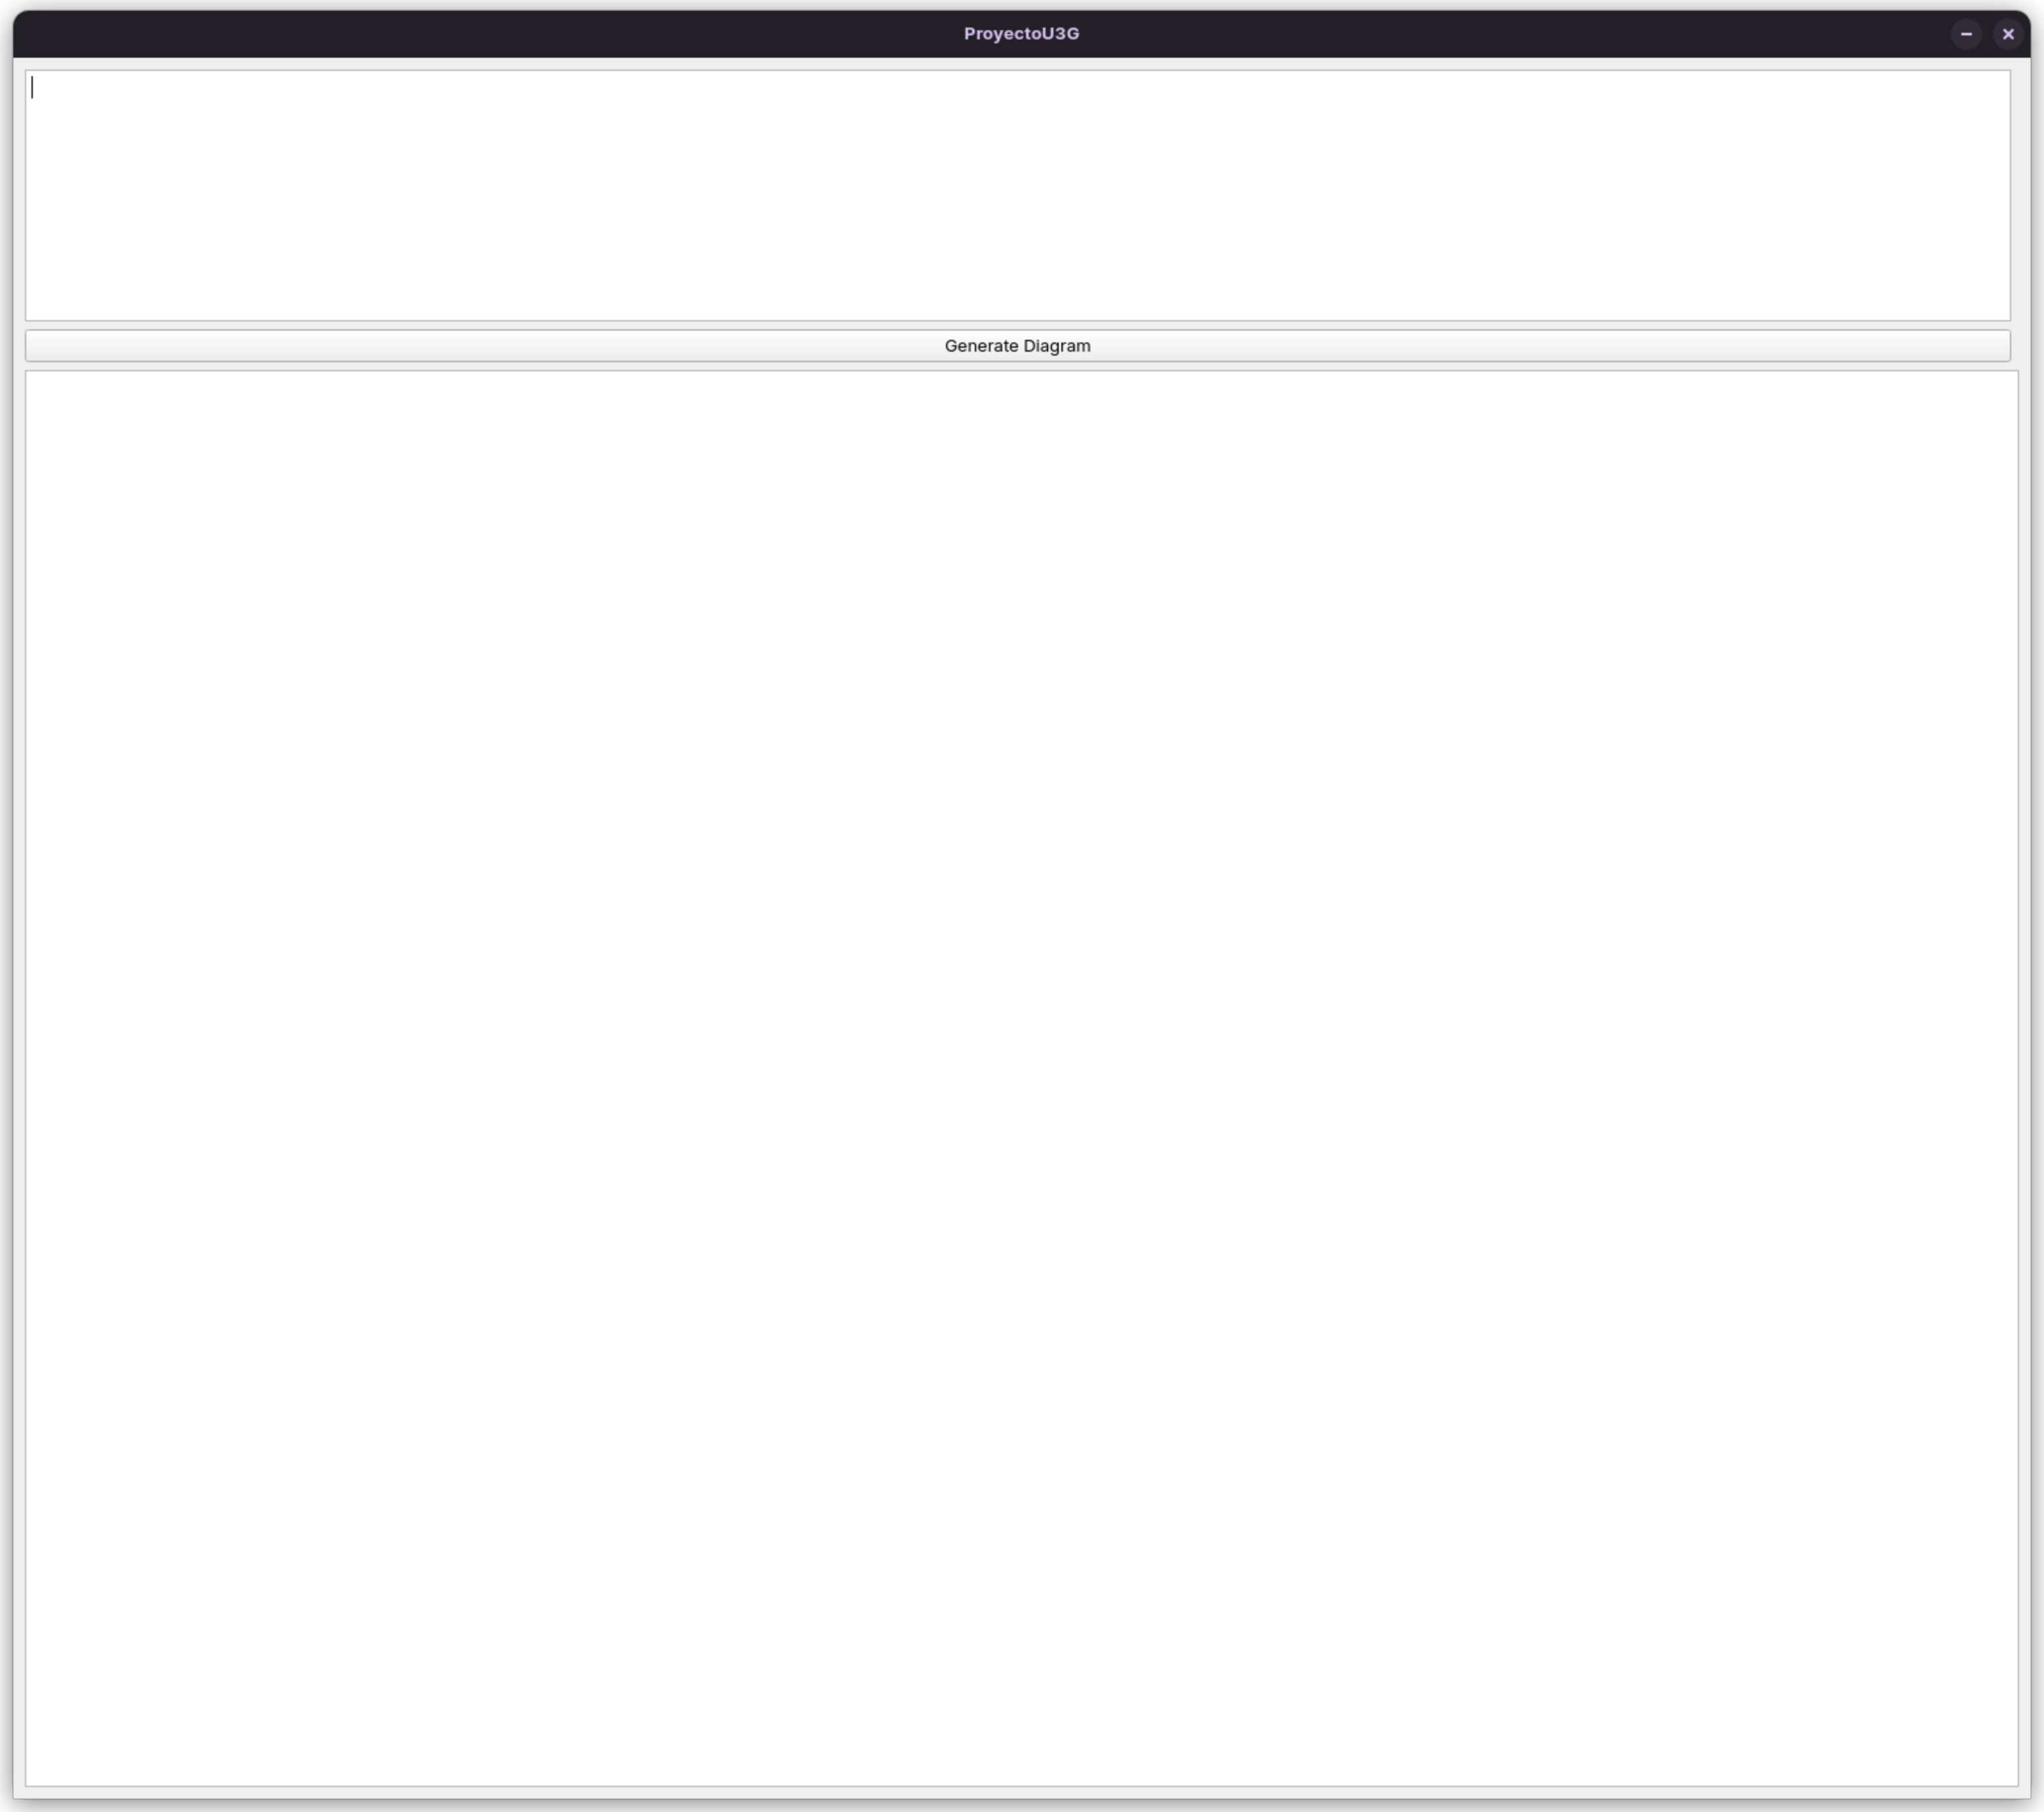
\includegraphics[width= 7cm]{imagen 1.png}
    \caption{Ejecución}
    \label{fig:ejecucion}
\end{figure}

El texto ingresado en la aplicación puede ser utilizado para generar un diagrama para la sintaxis de una consulta SQL \cite{sql} utilizando la sentencia SELECT. 

En la figura \ref{fig:ejemplo_1} hay un campo de texto con el esquema de la consulta SQL, que incluye varias cláusulas como SELECT, FROM, WHERE, GROUP BY, HAVING, ORDER BY, UNION, LIMIT y OFFSET. Cada una de estas cláusulas está representada en el diagrama de flujo por debajo del campo de texto, donde se organizan en bloques rectangulares conectados.
\begin{figure} [H]
    \centering
    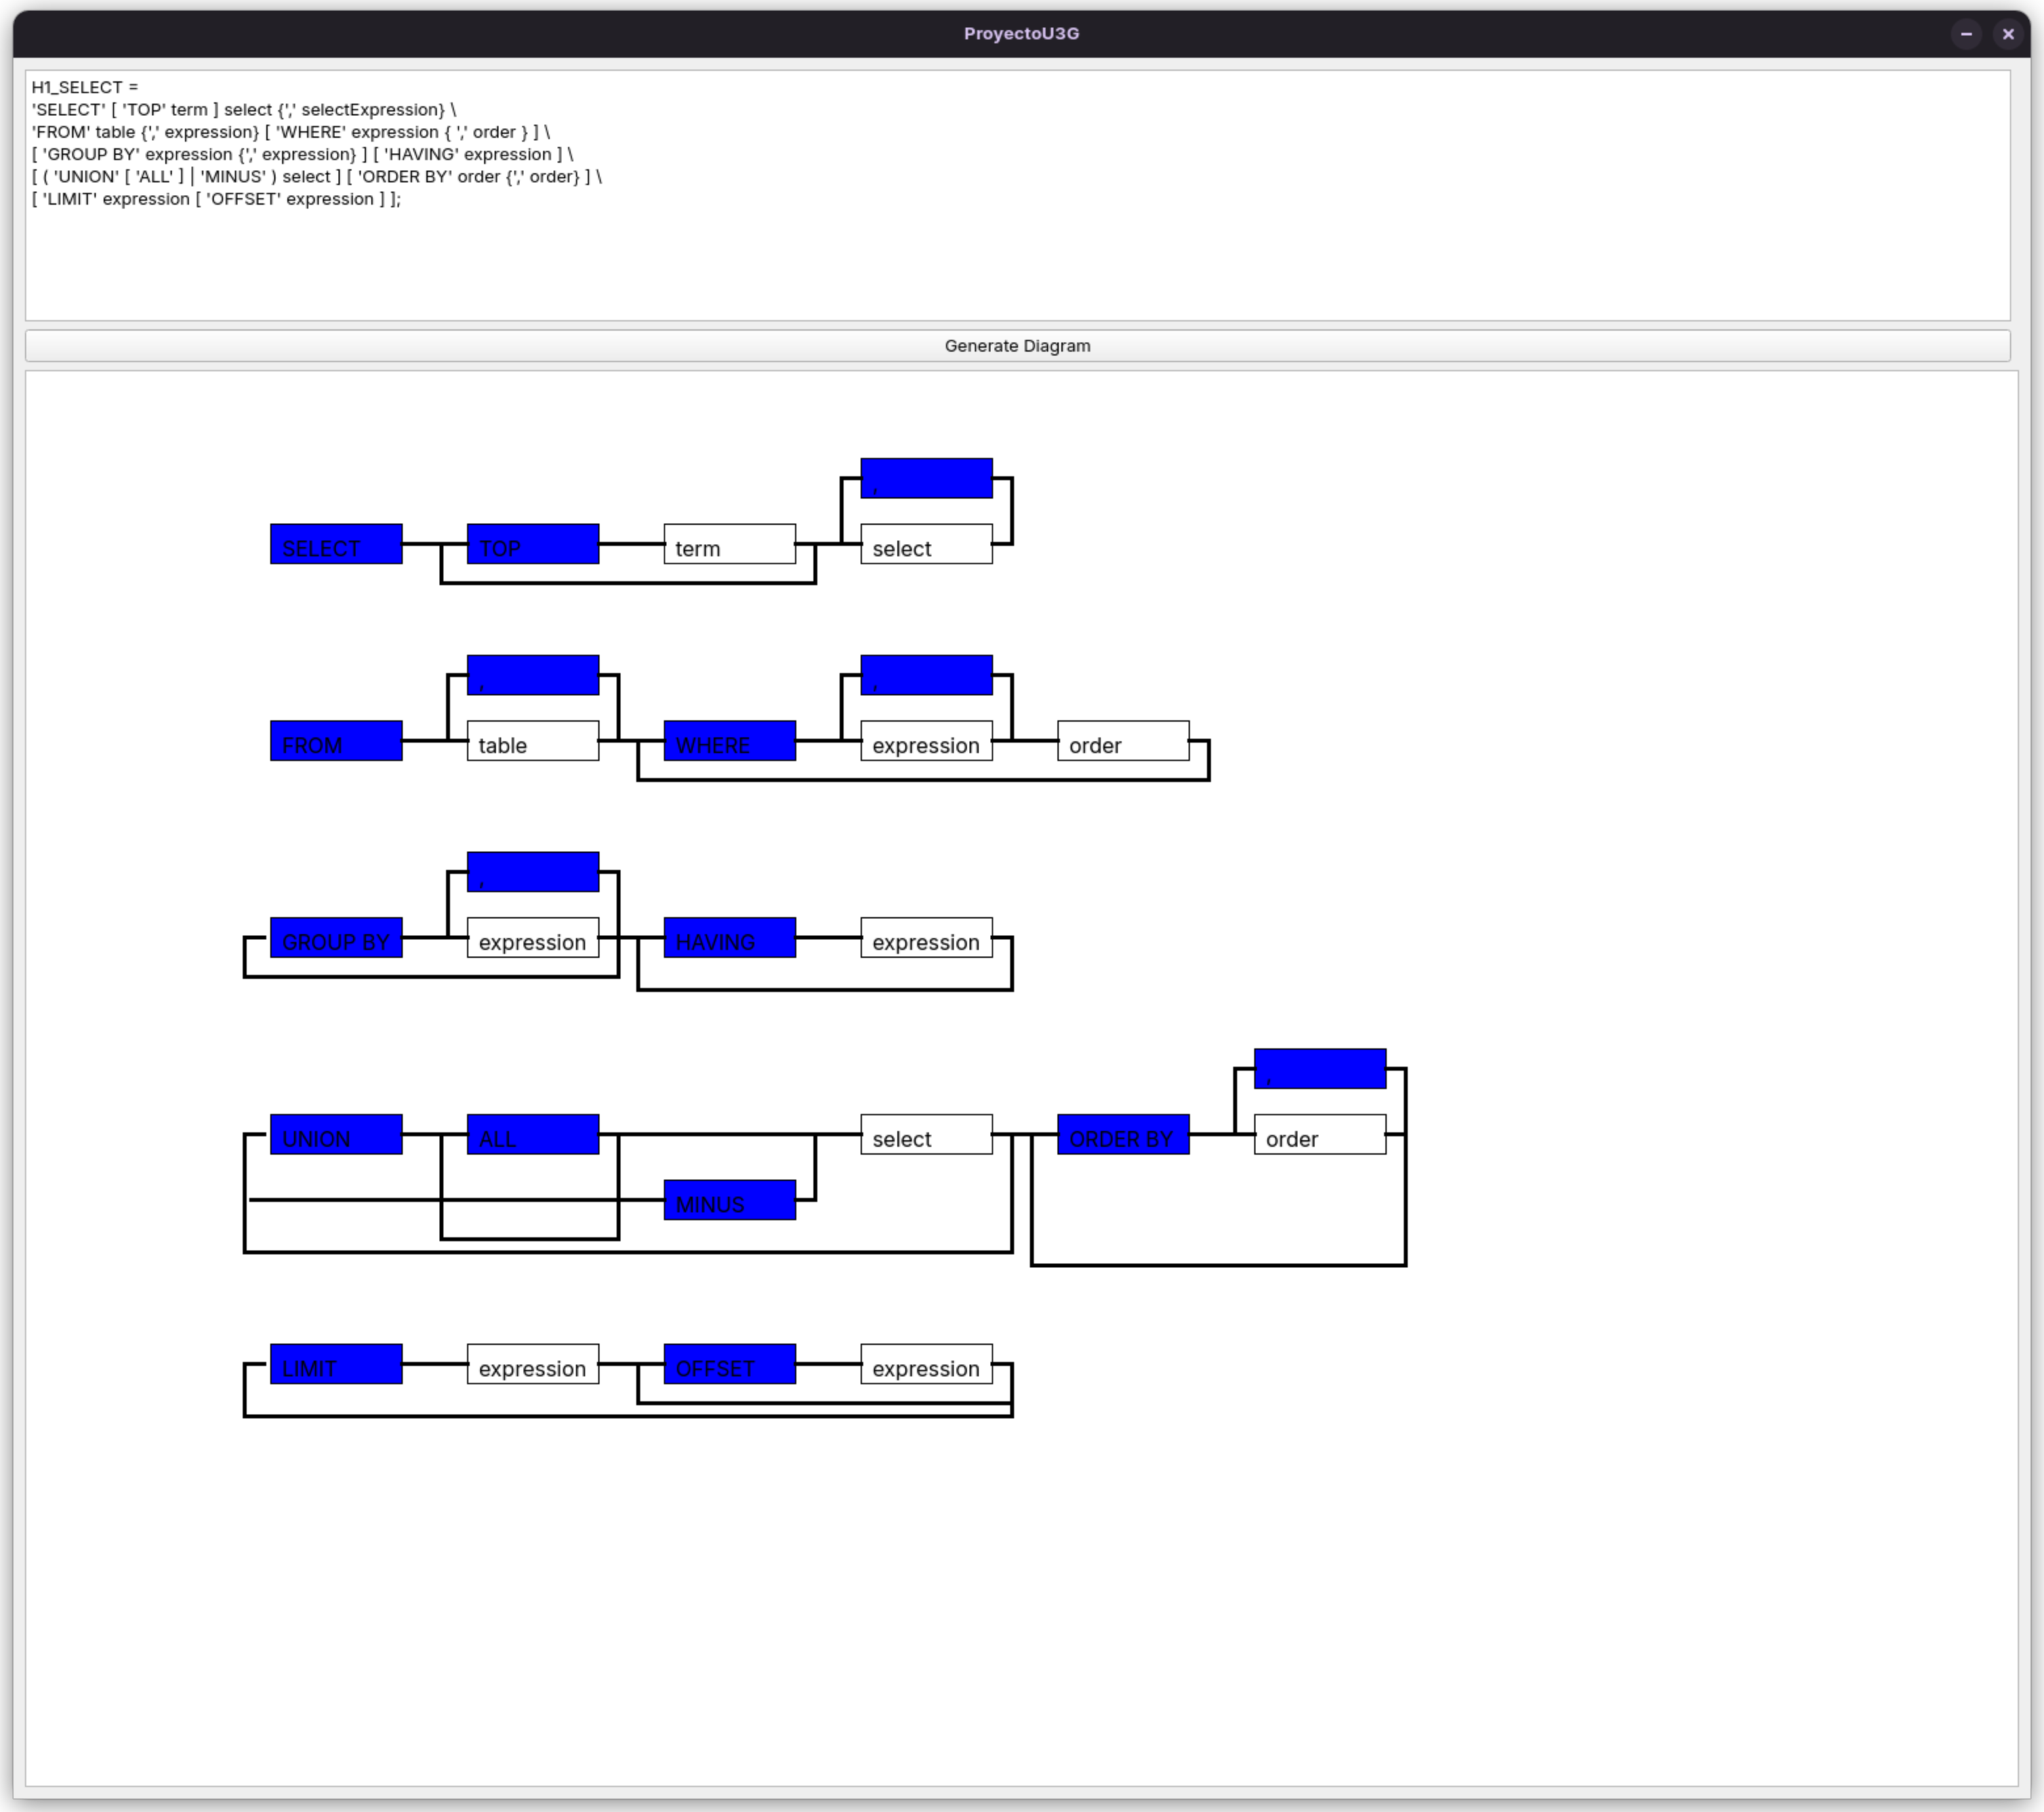
\includegraphics[width= 7cm]{imagen 2.png}
    \caption{Ingreso de cadena y diagrama generado. Ejemplo 1}
    \label{fig:ejemplo_1}
\end{figure}

La parte superior de la figura \ref{fig:ejemplo_2} tiene un área de texto con la sintaxis de la sentencia SQL, incluyendo palabras clave como DISTINCT, ALL, UNION, LIMIT, OFFSET, SAMPLE\_SIZE, y FOR UPDATE. Debajo, el diagrama de flujo estructura visualmente cómo se pueden combinar estas cláusulas en una consulta real. Por ejemplo, la cláusula SELECT puede ser seguida por TOP, DISTINCT, o ALL, indicando diferentes modos de seleccionar los datos. 

\begin{figure} [H]
    \centering
    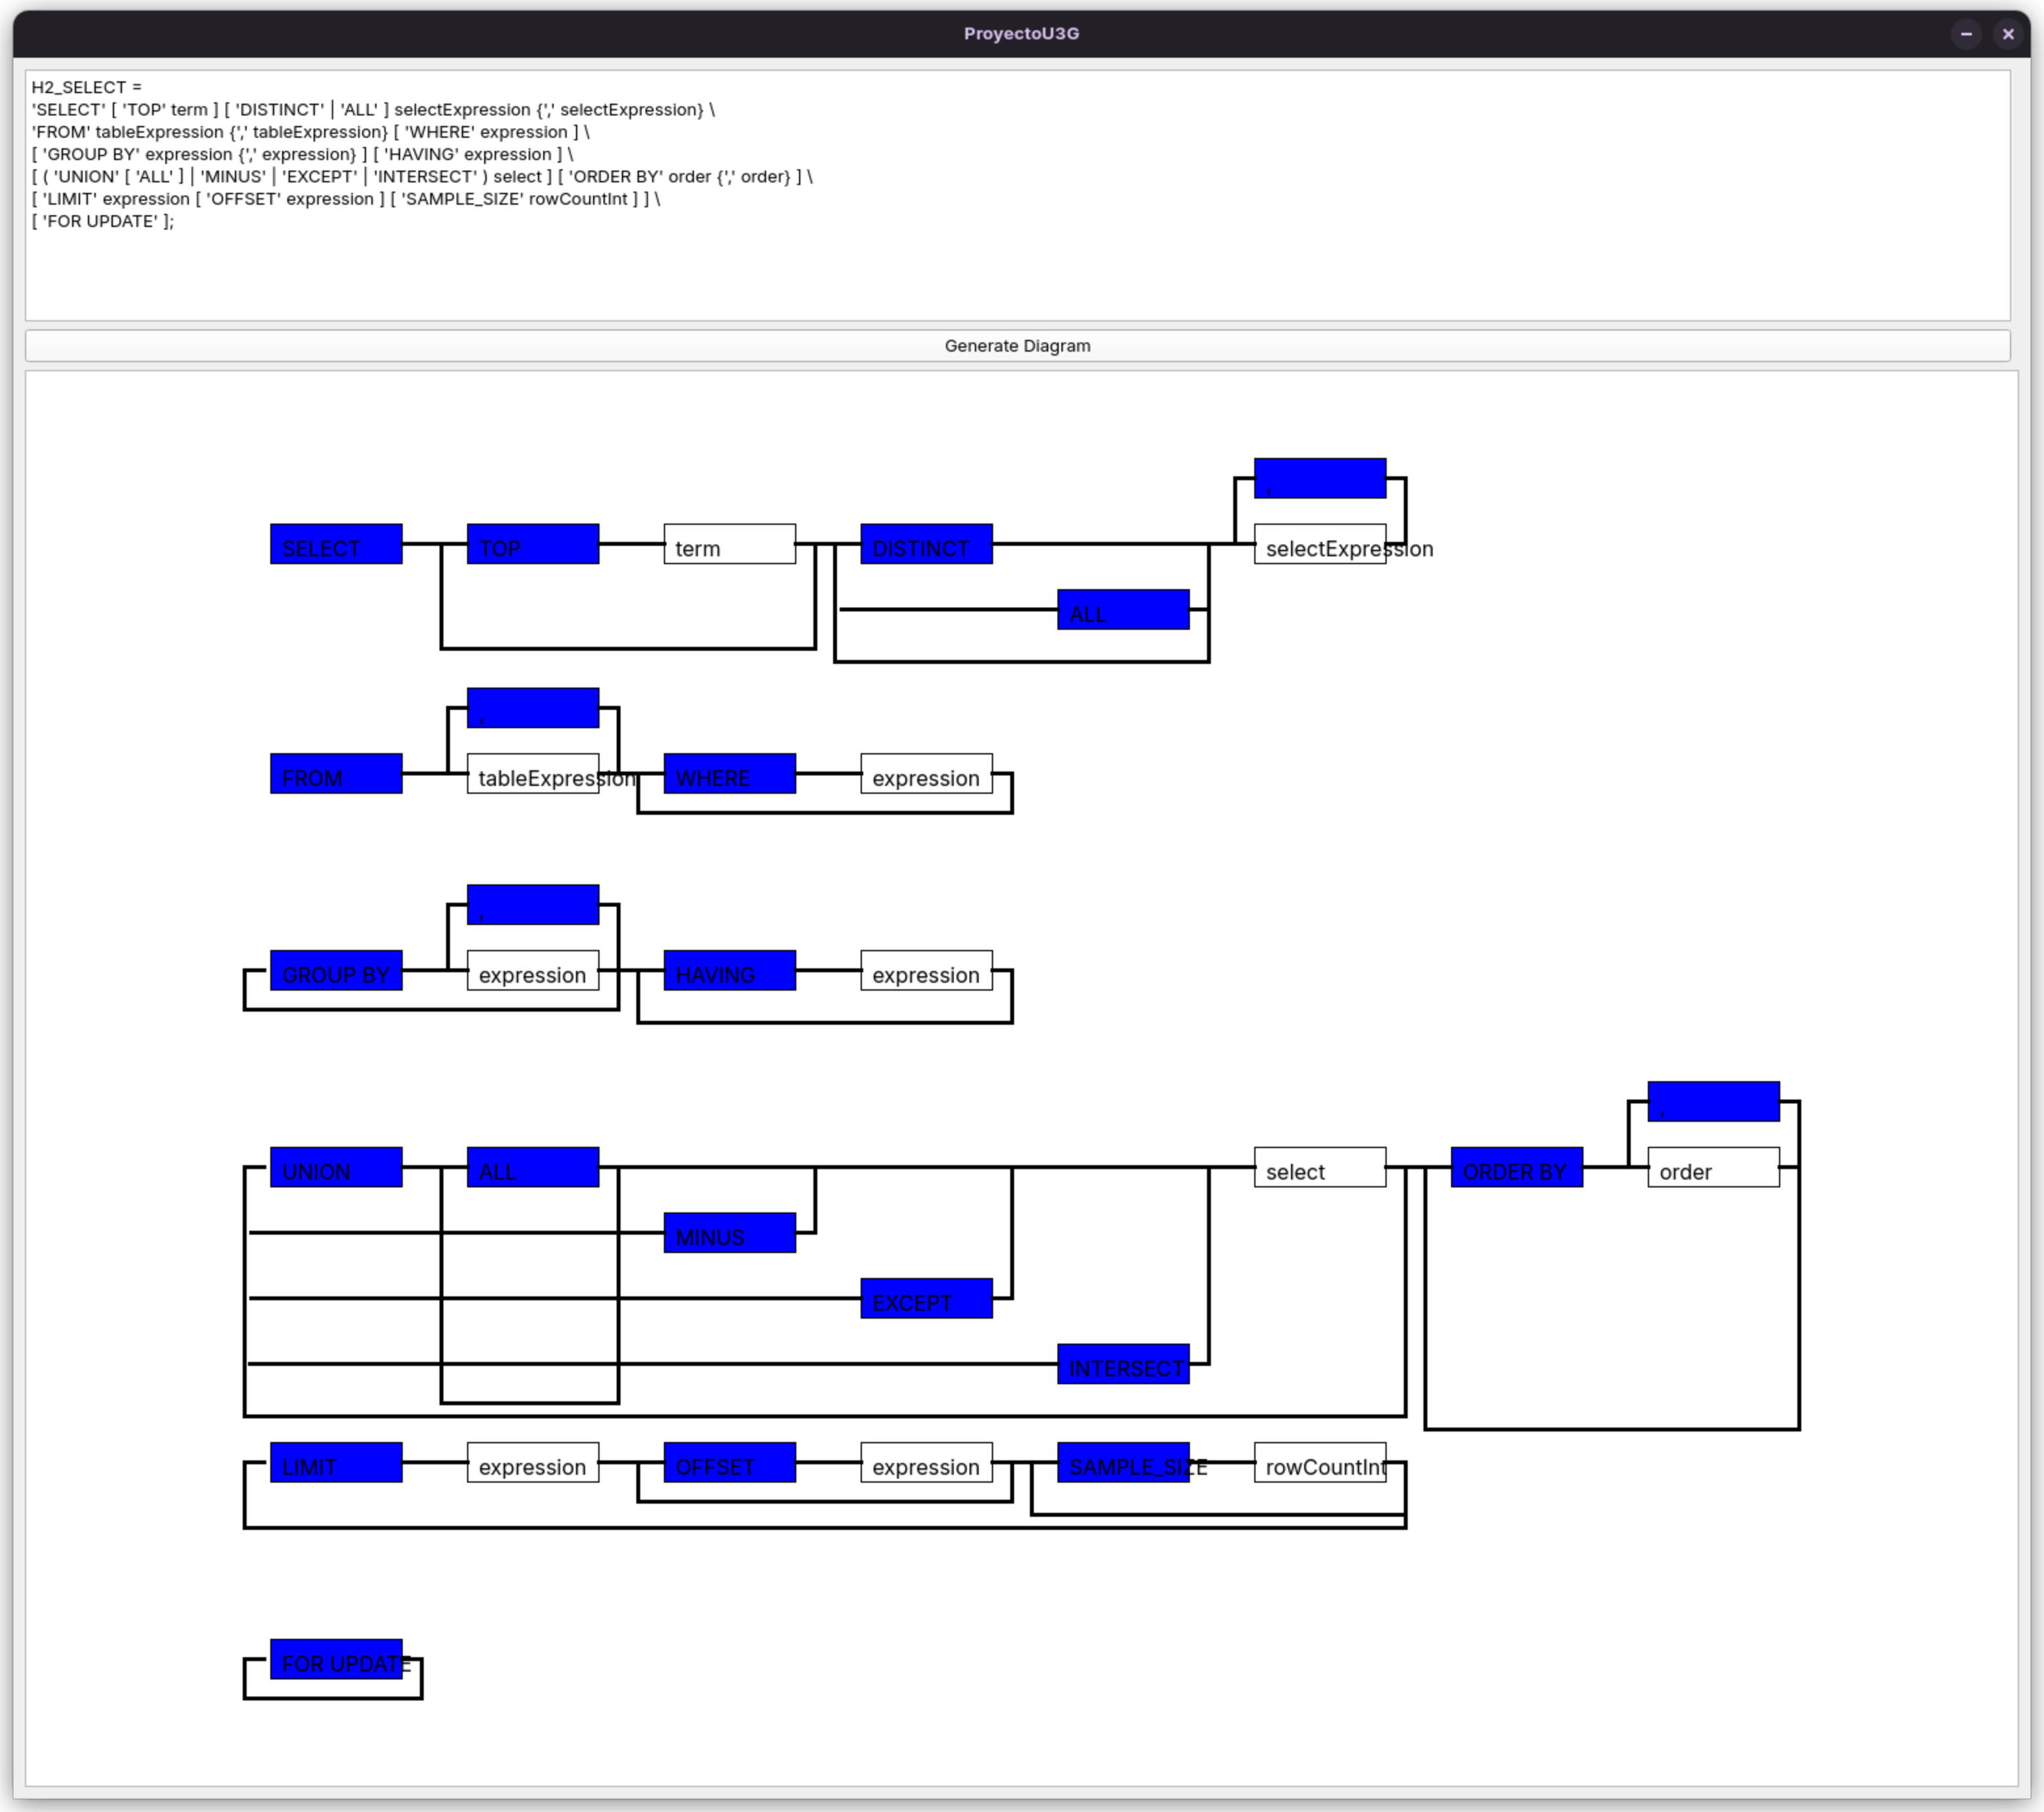
\includegraphics[width= 7cm]{imagen 3.png}
    \caption{Ingreso de cadena y diagrama generado. Ejemplo 2}
    \label{fig:ejemplo_2}
\end{figure}

En la figura \ref{fig:ejemplo_3}, se tiene una sintaxis en la cual describe detalladamente cómo debe estructurarse una instrucción SELECT o DELETE, proporcionando flexibilidad en términos de qué cláusulas y expresiones pueden ser incluidas o no, y en qué orden. Esta sintaxis sería útil para implementar un analizador sintáctico que pueda entender y procesar consultas SQL en un sistema de gestión de bases de datos o en un compilador SQL.

\begin{figure} [H]
    \centering
    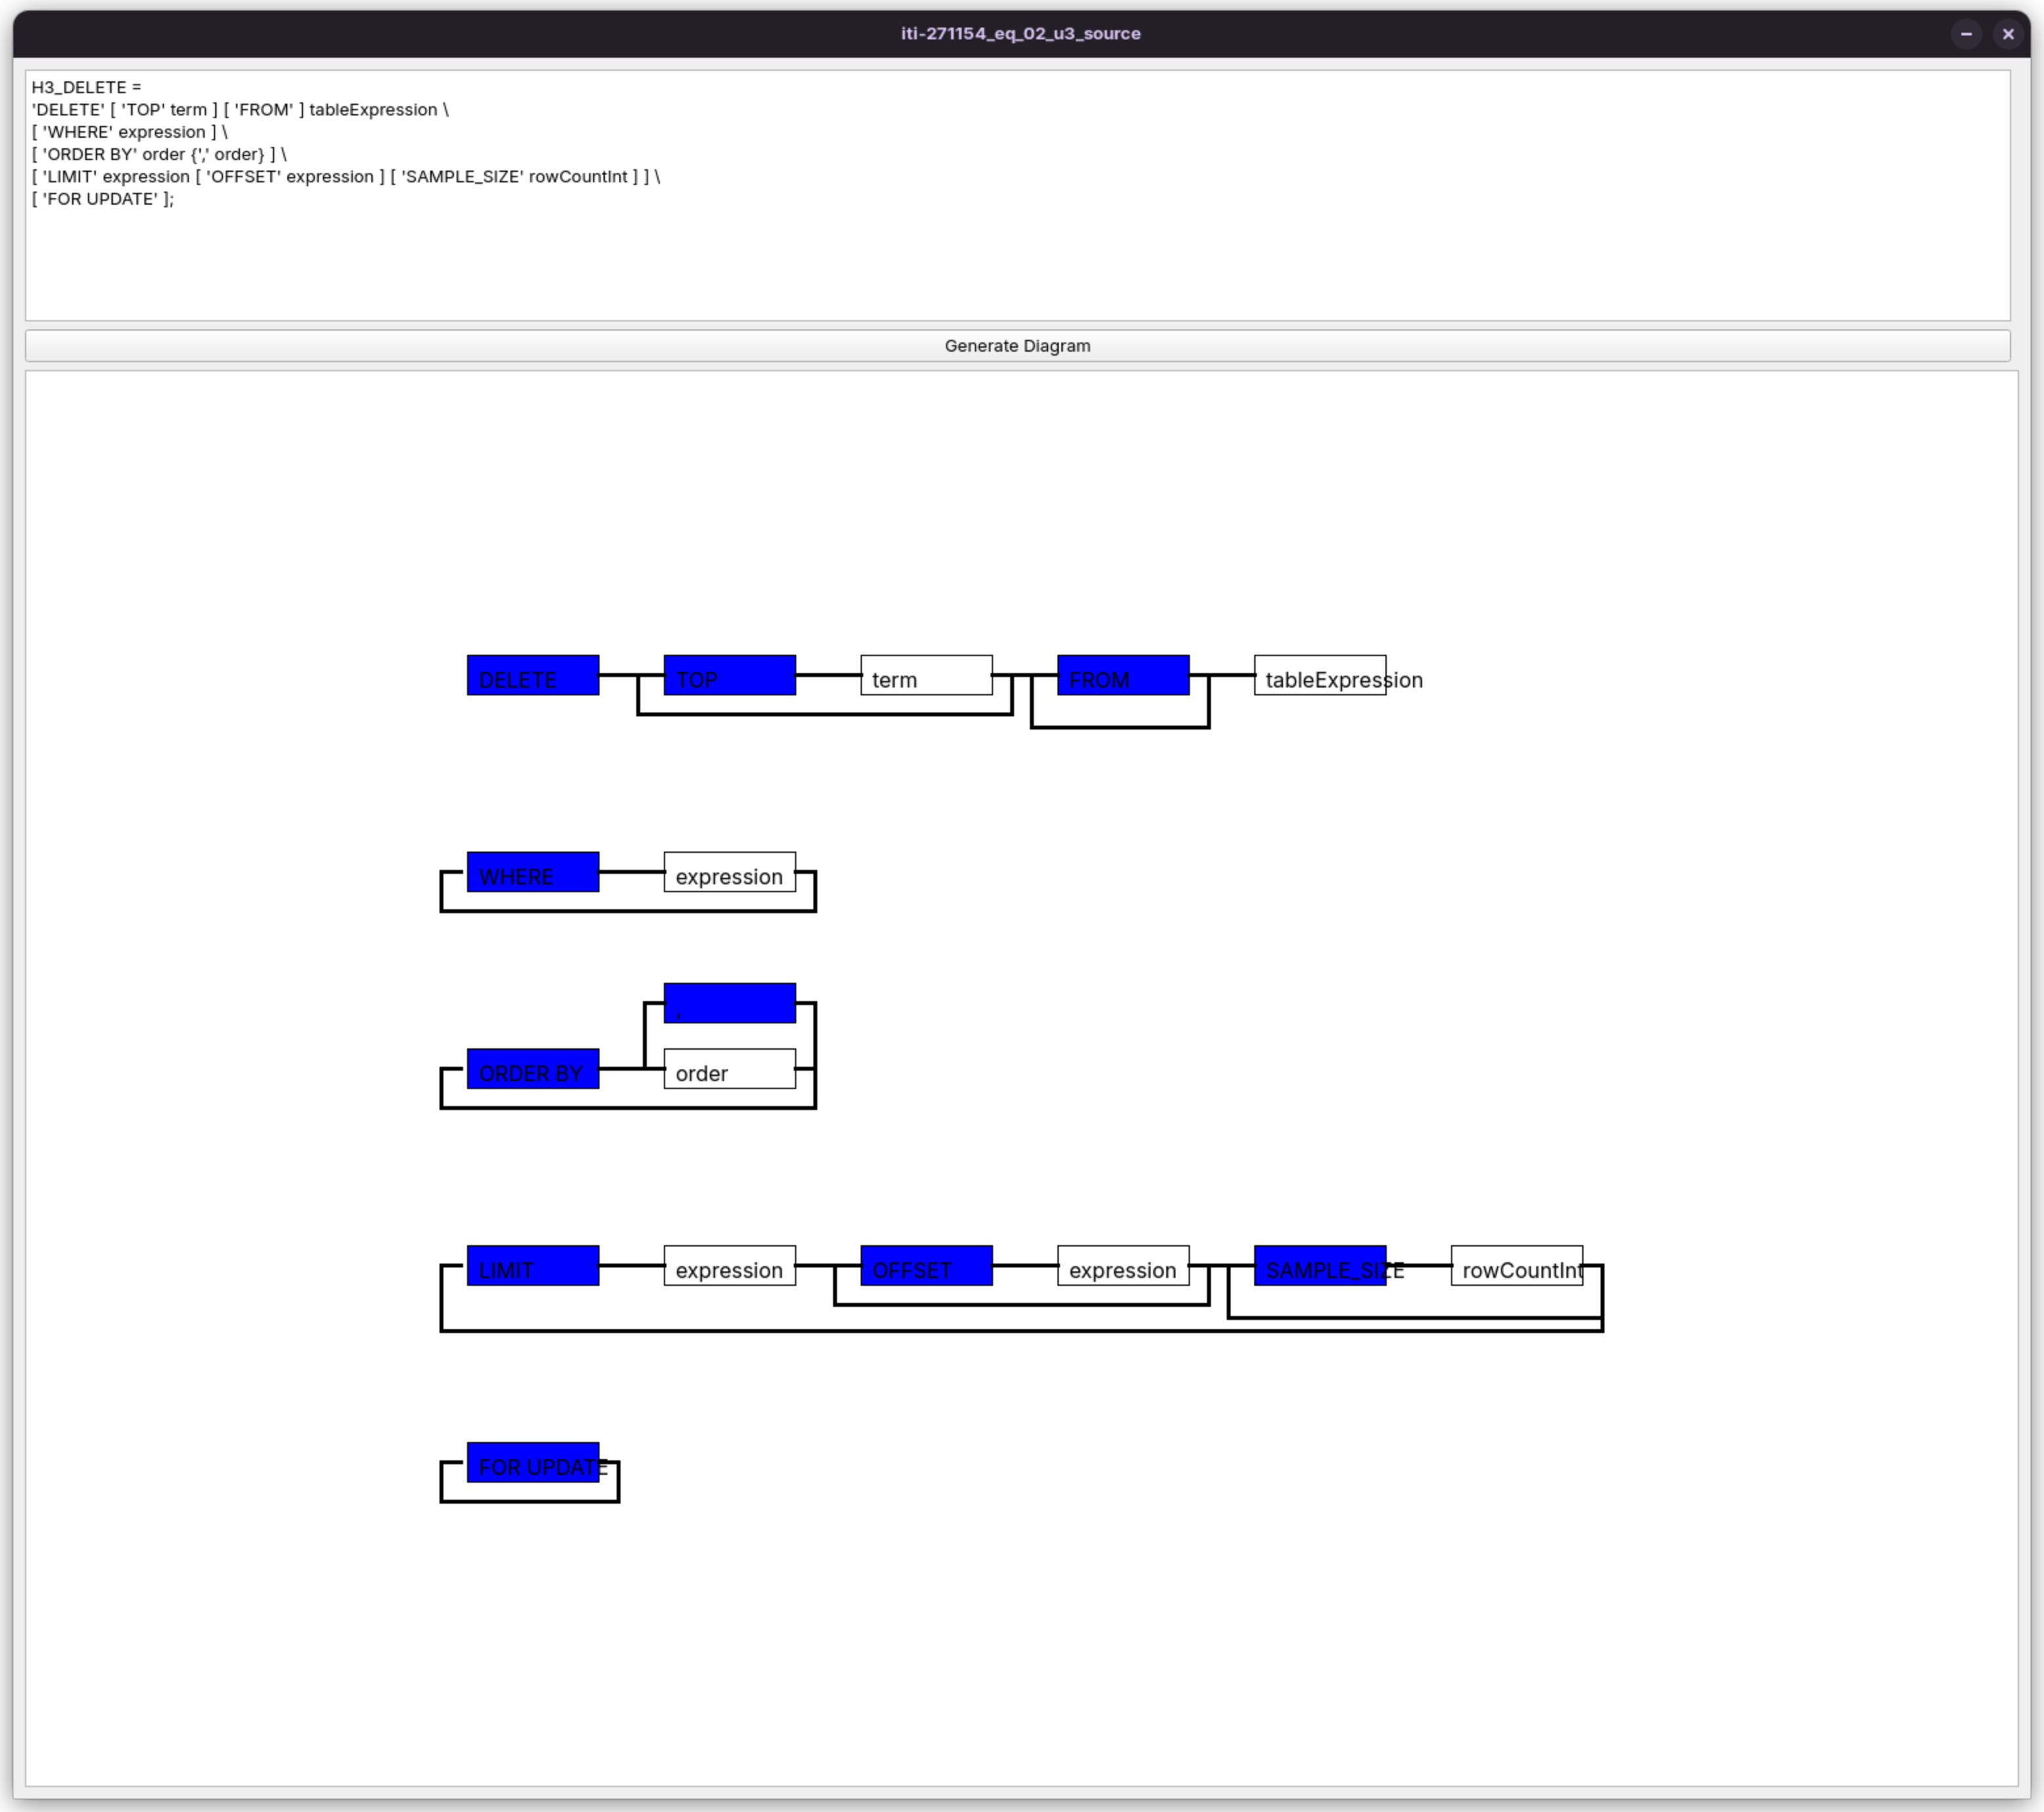
\includegraphics[width= 7cm]{imagen_4.png}
    \caption{Ingreso de cadena y diagrama generado. Ejemplo 3}
    \label{fig:ejemplo_3}
\end{figure}

\newpage
\section{Conclusión}
En conclusión, el proyecto "BFN to Railway" ha sido un esfuerzo colaborativo para desarrollar una aplicación de escritorio que cumple con el objetivo de convertir gramáticas definidas en notación BNF en diagramas de ferrocarril de manera dinámica. Utilizando el lenguaje de programación C++ y la biblioteca Qt5, se ha creado una interfaz interactiva que permite a los usuarios ingresar sus gramáticas y obtener visualizaciones gráficas claras y comprensibles de las mismas.

A lo largo del desarrollo del proyecto, se ha logrado implementar con éxito la generación de diagramas, la gestión de agrupaciones dentro de corchetes y la visualización adecuada de las producciones gramaticales. Aunque el proceso de desarrollo ha presentado desafíos y obstáculos, el equipo ha trabajado de manera colaborativa para superarlos y alcanzar los objetivos establecidos.

El programa resultante ofrece una herramienta útil para estudiantes y profesionales que trabajan con gramáticas formales, facilitando la comprensión y visualización de estructuras gramaticales complejas. Además, el proyecto ha brindado una oportunidad invaluable para aplicar los conocimientos teóricos adquiridos en la asignatura de Lenguajes y Autómatas en un contexto práctico y relevante.
\newpage
\addcontentsline{toc}{section}{Referencias} 
\printbibliography
%\balance



\end{document}
